%% LyX 2.3.1-1 created this file.  For more info, see http://www.lyx.org/.
%% Do not edit unless you really know what you are doing.
\documentclass[brazil,english,american]{beamer}
\usepackage[T1]{fontenc}
\usepackage[latin9]{inputenc}
\setcounter{secnumdepth}{4}
\setcounter{tocdepth}{1}
\usepackage{babel}
\usepackage{array}
\usepackage{booktabs}
\usepackage{amsmath}
\usepackage{amssymb}
\usepackage{graphicx}
\usepackage{setspace}
\usepackage{subscript}
\ifx\hypersetup\undefined
  \AtBeginDocument{%
    \hypersetup{unicode=true}
  }
\else
  \hypersetup{unicode=true}
\fi

\makeatletter

%%%%%%%%%%%%%%%%%%%%%%%%%%%%%% LyX specific LaTeX commands.
%% Because html converters don't know tabularnewline
\providecommand{\tabularnewline}{\\}

%%%%%%%%%%%%%%%%%%%%%%%%%%%%%% Textclass specific LaTeX commands.
% this default might be overridden by plain title style
\newcommand\makebeamertitle{\frame{\maketitle}}%
% (ERT) argument for the TOC
\AtBeginDocument{%
  \let\origtableofcontents=\tableofcontents
  \def\tableofcontents{\@ifnextchar[{\origtableofcontents}{\gobbletableofcontents}}
  \def\gobbletableofcontents#1{\origtableofcontents}
}

%%%%%%%%%%%%%%%%%%%%%%%%%%%%%% User specified LaTeX commands.
\usetheme{Warsaw}
% or ...

\setbeamercovered{transparent}
% or whatever (possibly just delete it)

\makeatother

\begin{document}
\title[Macroeconomic shocks and Regional Employment.]{Modeling How Macroeconomic Shocks Affect Regional Employment: Analyzing
the Brazilian Formal Labor Market using the Global VAR Approach.}
\author[Mar�al et. al. - Sao Paulo School of Economics ]{Emerson Fernandes Mar�al\\
Bruno Tebaldi\\
}
\institute[emerson.marcal@fgv.br]{Sao Paulo School of Economics, FGV \\
}

\makebeamertitle
%\pgfdeclareimage[height=0.5cm]{institution-logo}{cemap_logo}


%\logo{\pgfuseimage{institution-logo}}

\pgfdeclareimage[height=0.5cm]{institution-logo}{logo-cemap.png}


%\pgfdeclareimage[height=1.5cm]{institution-logo}{C:\Users\emerson.marcal\Dropbox\FGV\CEMAP\pesquisas\observatorio\TB-NFA-approach\apresentacao\FGV-seminario-2017-08-24\logo-cemap.png}



\logo{\pgfuseimage{institution-logo}}

\AtBeginSection[]{

  \frame<beamer>{ 

   \frametitle{Talking Points}   

  \tableofcontents[currentsection, currentsubsection] 

}

}

%\beamerdefaultoverlayspecification{<+->}
\begin{frame}{Talking points}
{\scriptsize{}}

{\scriptsize{}\tableofcontents{}}{\scriptsize\par}

{\scriptsize{}}{\scriptsize\par}
\end{frame}


\section{CEMAP: }
\begin{frame}{\foreignlanguage{brazil}{Center for Applied Macroeconomic Research - FGV}}
\begin{itemize}
\item Center for Applied Macroeconomic Research is part of Sao Paulo School
of Economics;
\item The main goal of the Center is to boost Applied Macroeconomic Research
at the School;
\item Our web-page is \href{http://www.cemap.fgv.br/}{www.cemap.fgv.br/};
\end{itemize}
\end{frame}

\begin{frame}{\foreignlanguage{brazil}{Our projects}}

\begin{itemize}
\item Observatory on Exchange Rate;
\item Forecast Lab;
\item Spatial Econometrics;
\item Time Series Econometrics;
\end{itemize}
\end{frame}


\section{Motivation}
\begin{frame}{Macroeconomics and Regional Data:}

\begin{itemize}
\item \textcolor{black}{Macroeconomic shocks affect sectors and regions
with different intensities and delays;}
\item \textcolor{black}{Population and economic activities tend to be clustered
in specific areas due economies of scale and agglomeration.}
\item \textcolor{black}{The population tends to be located near sea coast
compared with interior continental areas. }
\item \textcolor{black}{Sector activities tend to be concentrated in some
areas or cities. }
\end{itemize}
\end{frame}

\begin{frame}{Motivation}

\begin{itemize}
\item \textcolor{black}{Macroeconomic models tend to disregard regional
and spatial economic activity issues due to }
\begin{itemize}
\item \textcolor{black}{either their aggregate nature bias }
\item \textcolor{black}{or complexity of theme. }
\end{itemize}
\item \textcolor{black}{However for a specific region, it is important to
understand how economic activity variance can be decomposed into}
\begin{itemize}
\item \textcolor{black}{common factors (possibly macroeconomic factor) and }
\item \textcolor{black}{idiosyncratic factors;}
\end{itemize}
\end{itemize}
\end{frame}

\begin{frame}{Goals}

\begin{itemize}
\item \textcolor{black}{We want to model possible interaction between macroeconomic
shocks and regional employment dynamics;}
\item Assess possible different responses of regional employment to the
same shock;
\item Generate scenarios for regional employment evolution in Brazil bases
on a well specific time series model;
\end{itemize}
\end{frame}

\begin{frame}{Possible innovation}

\begin{itemize}
\item \textcolor{black}{Apply GVAR to link macroeconomic with regional dimension
in Brazil;}
\begin{itemize}
\item Deal with curse of dimensionality;
\end{itemize}
\item Use of IBGE Survey on economic links of Brazilian economy to construct
weights in GVAR;
\end{itemize}
\end{frame}


\section{Challenges and Methods}

\subsection{Global VAR}
\begin{frame}{Global VAR approach}

\begin{itemize}
\item Global autoregressive vector (GVAR) methodology was made by Pesaran,
Weiner and Schuermann (2004), and improved on by Dees, Mauro, Pesaran
and Smith (2007);
\item Chudik and Pesaran (2011) - Analyzed the curse of dimensionality in
the case of large dynamic linear systems. 
\item Infinite-dimensional VAR could be well approximated by a set of finite
dimensional small-scale models that can be consistently estimated
separately.
\item Spatial analysis application is a natural option of this framework;
\end{itemize}
\end{frame}

\begin{frame}{The Global VAR model as a two-step procedure}

\begin{itemize}
\item {\small{}First stage: Specific models of each region are estimated
conditioned on external influences from other regions.}{\small\par}

\begin{equation}
x_{it}=a_{i0}+a_{i1}t+\sum_{j=1}^{p_{i}}\Phi_{ij}x_{i,t-j}+\Lambda_{i0}x_{it}^{*}+\sum_{l=1}^{qi}\Lambda_{il}\text{\ensuremath{x}}_{\text{\ensuremath{i}}t-l}^{*}+u_{it}
\end{equation}

\[
x_{it}^{*}=\sum_{j=0}^{N}W_{ij}x_{jt}
\]

\item And they can be restated as:

\begin{equation}
A_{i0}W_{i}x_{t}=a_{i0}+a_{i1}t+\sum_{l=1}^{p}A_{il}W_{i}x_{t-l}+\epsilon_{t}
\end{equation}

\end{itemize}
\end{frame}

\begin{frame}{The Global VAR model as a two-step procedure}

\begin{itemize}
\item {\small{}Second Stage: The VAR models of each region are grouped into
a single Global VAR model.}{\small\par}
\end{itemize}
{\scriptsize{}
\[
G_{0}=\left[\begin{array}{c}
A_{00W_{0}}\\
A_{10W_{1}}\\
\vdots\\
A_{N0}W_{N}
\end{array}\right];\quad G_{l}=\left[\begin{array}{c}
A_{0lW_{0}}\\
A_{1lW_{1}}\\
\vdots\\
A_{Nl}W_{N}
\end{array}\right];a_{0}=\left[\begin{array}{c}
a_{00}\\
a_{10}\\
\vdots\\
a_{N0}
\end{array}\right];\quad a_{1}=\left[\begin{array}{c}
a_{01}\\
a_{11}\\
\vdots\\
a_{N1}
\end{array}\right];\quad\epsilon_{1}=\left[\begin{array}{c}
\epsilon_{0t}\\
\epsilon_{1t}\\
\vdots\\
\epsilon_{Nt}
\end{array}\right];
\]
}{\scriptsize\par}

{\scriptsize{}
\[
G_{0}x_{t}=a_{0}+a_{1}t+\sum_{l=1}^{p}G_{l}x_{t-l}+\epsilon_{t}
\]
\[
F_{i}=G_{0}^{-1}G_{i};\quad b_{0}=G_{0}^{-1}a_{0};\quad b_{1}=G_{0}^{-1}a_{1};\quad e_{t}=G_{0}^{-1}\epsilon_{t};
\]
}{\scriptsize\par}

{\scriptsize{}
\[
x_{t}=b_{o}+b_{1}t+\sum F_{i}x_{t-i}+e_{t}
\]
}{\scriptsize\par}
\end{frame}

\begin{frame}{How to choose the weights}

\begin{itemize}
\item {\small{}In macroeconomic apllications, share of trade or of the GDP
are natural choices}{\scriptsize{};}{\scriptsize\par}
\item In a spatial analysis weight can be function of distance;
\end{itemize}
\end{frame}


\subsection{Some references on labor market}
\begin{frame}{Selected papers on the subject}

\begin{itemize}
\item {\footnotesize{}Oliveira and Carneiro (2001) - Analysis of the dynamics
of the employment level of several Brazilian states in relation to
national employment with the objective of verifying a long term relationship.}{\footnotesize\par}
\item {\footnotesize{}Camila Kraide Kretzmann and Marina Silva da Cunha
(2009) - Analysis of the formal labor market between metropolitan
and non-metropolitan areas in Brazil.}{\footnotesize\par}
\item {\footnotesize{}Norbert Schanne (2015) - Analysis of the regional
labor market in Germany, focusing on forecasting regional labor markets.
She used the GVAR methodology to perform a prospective analysis of
the German economy.}{\footnotesize\par}
\item All these papers confirms the existence of links among regions;
\end{itemize}
\end{frame}


\section{Data}

\subsection{Database Description}

\begin{frame}{Brazilian Economy Structure}

\begin{columns}[t]
\selectlanguage{english}%

\column{7cm}

\selectlanguage{american}%
{\tiny{}}
\begin{figure}
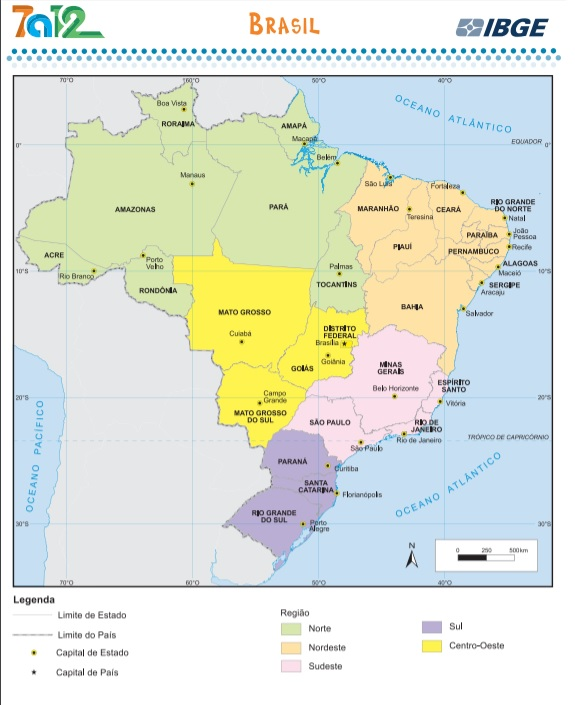
\includegraphics[width=3.5cm]{brazil-mapa}

{\scriptsize{}\caption{{\scriptsize{}Brazilian Regions}}
}{\scriptsize\par}
\end{figure}
{\tiny\par}
\selectlanguage{english}%

\column{4cm}
\selectlanguage{american}%
\begin{itemize}
\item {\scriptsize{}South and South East - Industrial, services and most
developed part of the country}{\scriptsize\par}
\item {\scriptsize{}North East - Agricultural and tourism}{\scriptsize\par}
\item {\scriptsize{}North - Agricultural - Amazon forest; }{\scriptsize\par}
\item {\scriptsize{}Central }\foreignlanguage{english}{{\scriptsize{}- }}{\scriptsize{}New
agricultural}\foreignlanguage{english}{{\scriptsize{} frontier;}}{\scriptsize\par}
\end{itemize}
\end{columns}

\end{frame}

\begin{frame}{Data}

{\scriptsize{}}%
\begin{tabular}{|>{\raggedright}p{2.5cm}||>{\raggedright}p{1.5cm}||>{\raggedright}p{2cm}||>{\raggedright}p{3cm}|}
\hline 
\textcolor{black}{\footnotesize{}Variable} & \textcolor{black}{\footnotesize{}Source} & \textcolor{black}{\footnotesize{}Frequency} & \textcolor{black}{\footnotesize{}Range}\tabularnewline
\hline 
\textcolor{black}{\footnotesize{}Brazilian Industrial Production} & \textcolor{black}{\footnotesize{}IBGE} & \textcolor{black}{\footnotesize{}Monthly} & \textcolor{black}{\footnotesize{}2004-01 to 2016-12}\tabularnewline
\hline 
\textcolor{black}{\footnotesize{}Admissions and Dismissals} & \textcolor{black}{\footnotesize{}CAGED} & \textcolor{black}{\footnotesize{}Monthly} & \textcolor{black}{\footnotesize{}2004-01 to 2016-12}\tabularnewline
\hline 
\textcolor{black}{\footnotesize{}Meso-regions and municipalities} & \textcolor{black}{\footnotesize{}IBGE} & \textcolor{black}{\footnotesize{}N/A} & \textcolor{black}{\footnotesize{}as of 2015}\tabularnewline
\hline 
\textcolor{black}{\footnotesize{}Connections between regions} & \textcolor{black}{\footnotesize{}IBGE} & \textcolor{black}{\footnotesize{}N/A} & \textcolor{black}{\footnotesize{}as of 2007}\tabularnewline
\hline 
\end{tabular}{\scriptsize\par}
\end{frame}

\begin{frame}{Some Graphics}

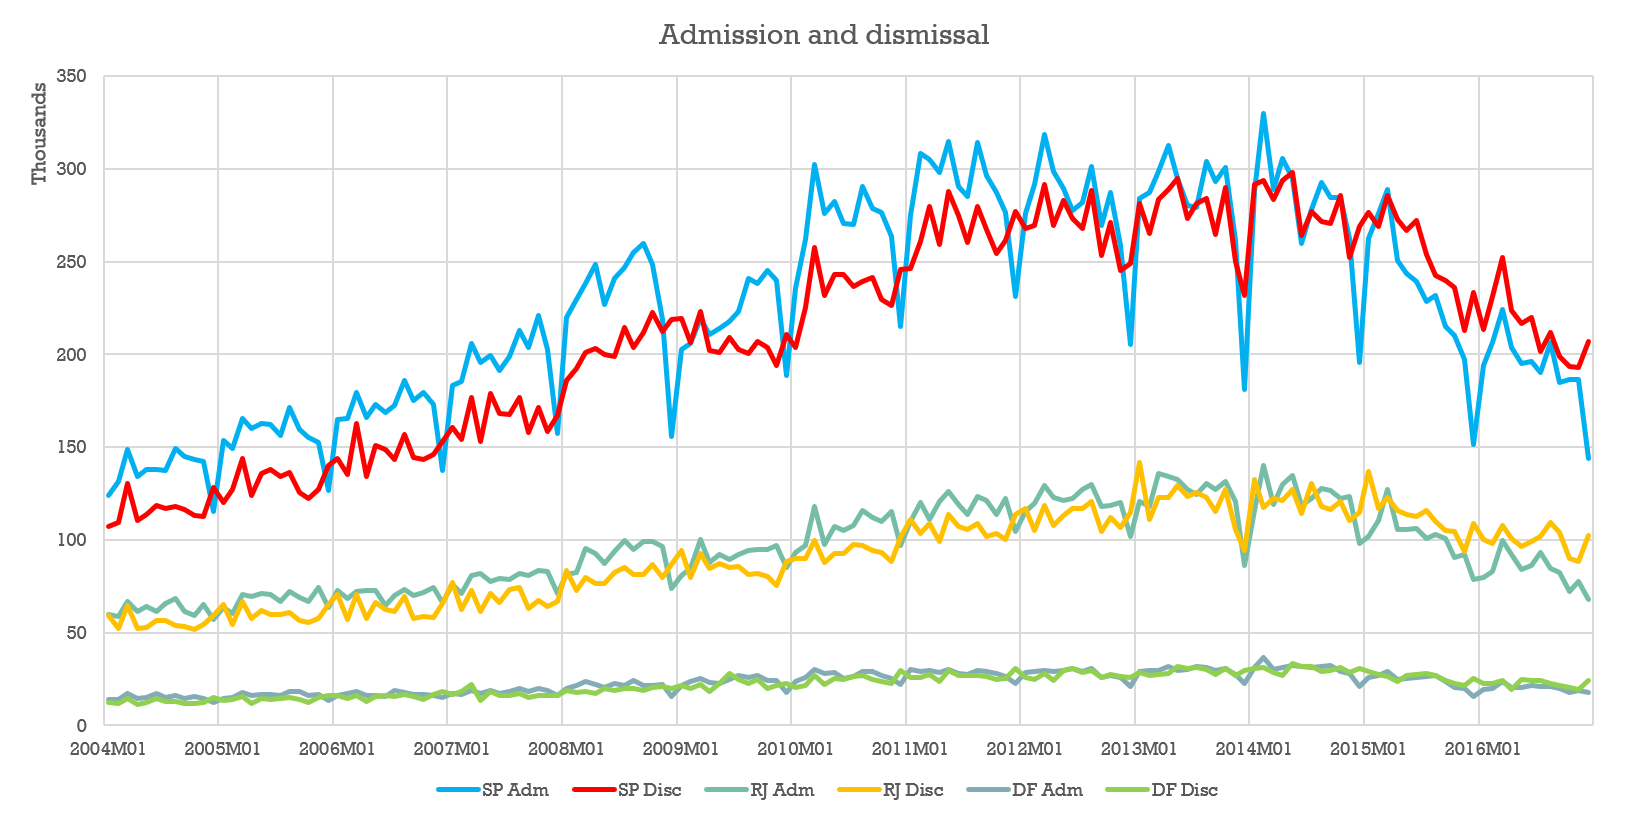
\includegraphics[scale=0.35]{fig2}
\end{frame}


\subsection{Model}
\begin{frame}{Model}

\begin{itemize}
\item The units in the model are the mesoregions defined by the Brazilian
Institute of Geography and Statistics.
\item The labor market variables are the numbers workers admitted and dismissed
from the labor market.

\[
x_{it}=\left[\begin{array}{c}
Adm_{it}\\
Dis_{it}
\end{array}\right];\quad x_{it}^{*}=\left[\begin{array}{c}
Adm_{it}^{*}\\
Dis_{it}^{*}
\end{array}\right]
\]

\[
Adm_{it}^{*}=\sum_{j=1}^{N}W_{ij}Adm_{jt}\quad Dis_{it}^{*}=\sum_{j=1}^{N}W_{ij}Dis_{jt}
\]

\end{itemize}
\end{frame}

\begin{frame}{Simple Macroeconomic Model}

\begin{itemize}
\item Macroeconomic model contains Brazilian production industrial index
and employment admissions and dismissals with feedback from regions:

\textrm{
\[
\omega_{t}=\left[ln(IndProd)\right]
\]
}

\[
\Delta\omega_{t}=\Phi_{\omega0}+\sum_{l=1}^{k1}\Phi_{\omega l}\Delta\omega_{t-l}+\sum_{l=1}^{k_{2}}\Lambda_{\omega l}\Delta x_{i,t-l}^{*}+\eta_{\omega t}
\]

\end{itemize}
\end{frame}

\begin{frame}{Our weight matrix choice}

\begin{columns}[t]
\selectlanguage{english}%

\column{6cm}

\selectlanguage{american}%
{\tiny{}}
\begin{figure}
{\tiny{}}%
\begin{tabular}{r}
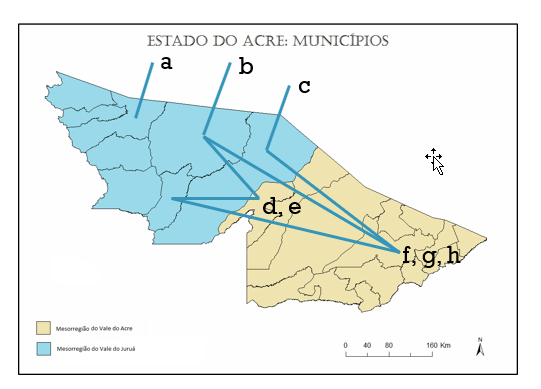
\includegraphics[width=3cm]{fig1}\tabularnewline
\end{tabular}{\tiny\par}

{\scriptsize{}\caption{{\scriptsize{}Response to changes in growth of industrial production}}
}{\scriptsize\par}
\end{figure}
{\tiny\par}
\selectlanguage{english}%

\column{3cm}
\selectlanguage{american}%
\begin{itemize}
\item {\scriptsize{}Survey of Brazilian Bureau of Geographic and Statistics
on economic links of regions;}{\scriptsize\par}
\item {\scriptsize{}Links available at all municipalities;}{\scriptsize\par}
\end{itemize}
\end{columns}

\begin{singlespace}
{\scriptsize{}
\[
W_{blue}=\frac{\left[\begin{array}{ccc}
c_{i1} & \dots & c_{iN}\end{array}\right]}{\sum_{j=1}^{N}c_{ij}}\quad W_{blue}=\frac{\left[\begin{array}{ccc}
5 &  & 3\end{array}\right]}{8}=\left[\begin{array}{cc}
0.625 & 0.375\end{array}\right]
\]
}{\scriptsize\par}
\end{singlespace}
\end{frame}


\subsection{Model details and specification}
\begin{frame}{Results}
\begin{itemize}
\item 137 specific models were specified.
\begin{itemize}
\item Domestic variables: 98 models with lag 2 and 39 models with lag 1
\item Foreign variables: 91 models with lag 2 and 46 models with lag 1.
\item 9 models with 1 cointegration relation and 128 models with 2 cointegration
relations.
\end{itemize}
\item Weak exogeneity status are satisfied for most of units;
\end{itemize}
\end{frame}


\section{Our Results}

\subsection{Employment Dynamics}
\selectlanguage{english}%
\begin{frame}{\foreignlanguage{american}{Brazilian Five Regions Response}}
\selectlanguage{american}%
\begin{columns}[t]
\selectlanguage{english}%

\column{8cm}

\selectlanguage{american}%
{\tiny{}}
\begin{table}
{\tiny{}}%
\begin{tabular}{rr}
\includegraphics[width=3cm]{\string"Figure2-a v2\string".png} & \includegraphics[width=3cm]{\string"Figure2-b v2\string".png}\tabularnewline
\includegraphics[width=3cm]{\string"Figure2-c v2\string".png} & \includegraphics[width=3cm]{\string"Figure2-d v2\string".png}\tabularnewline
\end{tabular}{\tiny\par}

{\scriptsize{}\caption{{\scriptsize{}Response to changes in growth of industrial production}}
}{\scriptsize\par}
\end{table}
{\tiny\par}
\selectlanguage{english}%

\column{3cm}
\selectlanguage{american}%
\begin{itemize}
\item {\scriptsize{}South (0.18) }{\scriptsize\par}
\item {\scriptsize{}North East (0.16) }{\scriptsize\par}
\item {\scriptsize{}South East (0.1) }{\scriptsize\par}
\item {\scriptsize{}North (0.06) }{\scriptsize\par}
\item {\scriptsize{}Central (0.06)}\foreignlanguage{english}{{\scriptsize{};}}{\scriptsize\par}
\end{itemize}
\end{columns}

\end{frame}
\selectlanguage{american}%

\selectlanguage{english}%
\begin{frame}{\foreignlanguage{american}{Southeast States Response}}
\selectlanguage{american}%
\begin{columns}[t]
\selectlanguage{english}%

\column{8cm}

\selectlanguage{american}%
{\tiny{}}
\begin{table}
{\tiny{}}%
\begin{tabular}{rr}
\includegraphics[width=3cm]{\string"Figure3-a v2\string".png} & \includegraphics[width=3cm]{\string"Figure3-b v2\string".png}\tabularnewline
\includegraphics[width=3cm]{\string"Figure3-c v2\string".png} & \includegraphics[width=3cm]{\string"Figure3-d v2\string".png}\tabularnewline
\end{tabular}{\tiny\par}

{\scriptsize{}\caption{{\scriptsize{}Response to changes in growth of industrial production}}
}{\scriptsize\par}
\end{table}
{\tiny\par}
\selectlanguage{english}%

\column{3cm}
\selectlanguage{american}%
\begin{itemize}
\item {\footnotesize{}Rio de janeiro (0.19) }{\footnotesize\par}
\item {\footnotesize{}Espirito Santo (0.09) }{\footnotesize\par}
\item {\footnotesize{}S�o Paulo (0.08) }{\footnotesize\par}
\item {\footnotesize{}Minas Gerais (0.07)}\foreignlanguage{english}{{\scriptsize{};}}{\scriptsize\par}
\end{itemize}
\end{columns}

\end{frame}
\selectlanguage{american}%

\selectlanguage{english}%
\begin{frame}{\foreignlanguage{american}{Selected meso regions}}
\selectlanguage{american}%
\begin{columns}[t]
\selectlanguage{english}%

\column{8cm}

\selectlanguage{american}%
{\tiny{}}
\begin{table}
{\tiny{}}%
\begin{tabular}{rr}
\includegraphics[width=3cm]{\string"Figure5-a v2\string".png} & \includegraphics[width=3cm]{\string"Figure5-b v2\string".png}\tabularnewline
\includegraphics[width=3cm]{\string"Figure5-c v2\string".png} & \includegraphics[width=3cm]{\string"Figure5-d v2\string".png}\tabularnewline
\end{tabular}{\tiny\par}

{\scriptsize{}\caption{{\scriptsize{}Response to changes in growth of industrial production}}
}{\scriptsize\par}
\end{table}
{\tiny\par}
\selectlanguage{english}%

\column{3cm}
\selectlanguage{american}%
\begin{itemize}
\item {\footnotesize{}Rio de Janeiro (0.19) }{\footnotesize\par}
\item {\footnotesize{}Porto Alegre (0.19) }{\footnotesize\par}
\item {\footnotesize{}Belo Horizonte (0.17) }{\footnotesize\par}
\item {\footnotesize{}S�o Paulo (0.16) }{\footnotesize\par}
\item {\footnotesize{}C. Goi�s (0.07)}{\footnotesize\par}
\item {\footnotesize{}Salvador (0.11)}{\footnotesize\par}
\end{itemize}
\end{columns}

\end{frame}
\selectlanguage{american}%

\selectlanguage{english}%
\begin{frame}{\foreignlanguage{american}{Selected Mesoregions}}
\selectlanguage{american}%
\begin{columns}[t]
\selectlanguage{english}%

\column{8cm}

\selectlanguage{american}%
{\tiny{}}
\begin{table}
{\tiny{}}%
\begin{tabular}{rr}
\includegraphics[width=3cm]{\string"Figure4-a v2\string".png} & \includegraphics[width=3cm]{\string"Figure4-b v2\string".png}\tabularnewline
\includegraphics[width=3cm]{\string"Figure4-c v2\string".png} & \includegraphics[width=3cm]{\string"Figure4-d v2\string".png}\tabularnewline
\end{tabular}{\tiny\par}

{\scriptsize{}\caption{{\scriptsize{}Response to changes in growth of industrial production}}
}{\scriptsize\par}
\end{table}
{\tiny\par}
\selectlanguage{english}%

\column{3cm}
\selectlanguage{american}%
\begin{itemize}
\item {\footnotesize{}Porto Alegre (0.19) }{\footnotesize\par}
\item {\footnotesize{}S�o Paulo (0.16) }{\footnotesize\par}
\item {\footnotesize{}C. Goi�s (0.07) }{\footnotesize\par}
\item {\footnotesize{}Borborema (0.02) }{\footnotesize\par}
\item {\footnotesize{}Jequit. (0.02)}\foreignlanguage{english}{{\scriptsize{};}}{\scriptsize\par}
\end{itemize}
\end{columns}

\end{frame}
\selectlanguage{american}%


\subsection{Conditional Forecast Exercise}
\begin{frame}{Scenario for growth}
\begin{itemize}
\item Several scenarios were estimated to assess the impact of industrial
production on the labor market.
\begin{itemize}
\item Annual growth of 0\%: A negative employment balance for at least the
next 8 years.
\item Annual growth of 2\%: A positive accumulated balance of 2.5 million
job positions for 8 years ahead.
\item Higher growth scenarios (4\%, 6\% and 8\%) show significant improvements
in the labor market.
\end{itemize}
\end{itemize}
\end{frame}
\selectlanguage{english}%

\selectlanguage{american}%
\begin{frame}{Dynamics of units}

\begin{itemize}
\item \href{file:4PercentGrowthtoPIM.mp4}{VIDEO}
\end{itemize}
\end{frame}

\begin{frame}{Conditional predictions from different scenarios}

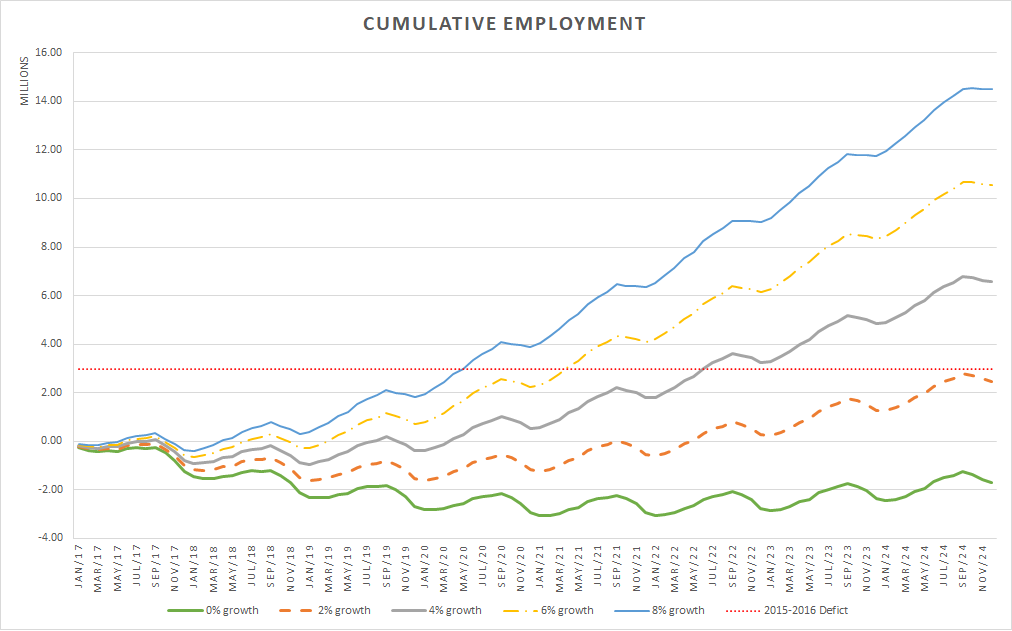
\includegraphics[width=9cm]{forecast-gvar}
\end{frame}

\begin{frame}{Forecasts vs. Outcome}

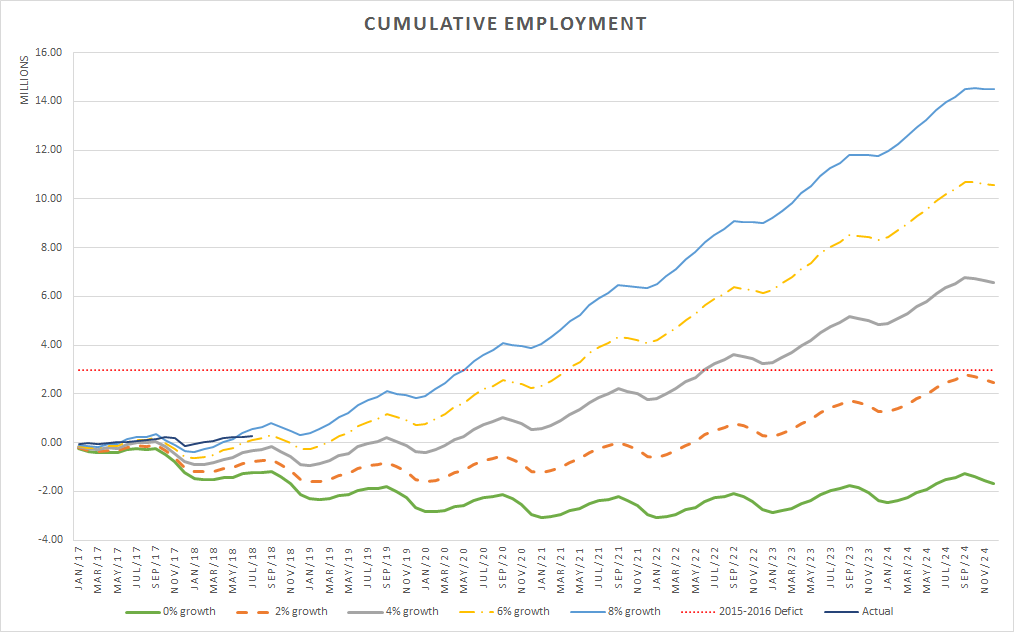
\includegraphics[width=9cm]{forecast-actual-gvar-2}
\end{frame}


\section{Limitations and Possible Extensions}
\begin{frame}{Limitations}
\begin{itemize}
\item Macroeconomic model can be improved to incorporate more variables
and disentangle possible different types of shocks;
\item Different weights strategies can be tried and compared;
\item Evaluation of forecast performance.
\end{itemize}
\end{frame}

\begin{frame}{Extensions}
\begin{itemize}
\item Work at higher disaggregated level but ``municipality split epidemia''
in Brazil must be addressed - Comparable minimum areas;
\item Models can be improved for each unity using \textit{Autometrics} algorithm
similar to Ericsson et al. (2012);
\item Using MINIMAL algorithm to unveil cointegration relationship among
cities to construct a ``expanded'' GVAR; 
\end{itemize}
\end{frame}


\section{A closer look on the benefits of Automatic Selection}

\subsection{Macroeconomic Model}
\begin{frame}{\foreignlanguage{english}{Small Macro Model}}
\begin{itemize}
\item Starting Point:
\begin{itemize}
\item VARX with twelve lagas for all variables plus error correction terms;
\item Centered Seasonal Dummies;
\end{itemize}
\end{itemize}
\selectlanguage{english}%
X\textsubscript{1} - Net Employment; 

X\textsubscript{2} - Dismissals;

X\textsubscript{3} - $\Delta$ ln Industrial Production;

X\textsubscript{4} -$\Delta$ ln Selic
\end{frame}
\selectlanguage{american}%

\begin{frame}{\foreignlanguage{english}{Instability Points}}

DI: First Difference Impulse Dummy

I: Impulse Dummy

SI: Step Dummy
\begin{itemize}
\item {\tiny{}DI:2001(12)}{\tiny\par}
\item {\tiny{}I:2003(3) }{\tiny\par}
\item {\tiny{}I:2008(12) }{\tiny\par}
\item {\tiny{}I:2018(6) }{\tiny\par}
\item {\tiny{}S1:2012(2) }{\tiny\par}
\item {\tiny{}S1:2012(3) }{\tiny\par}
\item {\tiny{}S1:2012(12) }{\tiny\par}
\item {\tiny{}S1:2013(1) }{\tiny\par}
\item {\tiny{}S1:2013(11) }{\tiny\par}
\item {\tiny{}S1:2013(12) }{\tiny\par}
\item {\tiny{}S1:2014(2)}{\tiny\par}
\end{itemize}
\end{frame}

\begin{frame}{\foreignlanguage{english}{Temporal Sequence}}

\selectlanguage{english}%
{\tiny{}}%
\begin{tabular}{llllll}
\hline 
{\tiny{}Past } & {\tiny{}-> } & {\tiny{}Present } & {\tiny{}Statistics } & {\tiny{}Distribution } & {\tiny{}p-value}\tabularnewline
\hline 
{\tiny{} X}\textsubscript{1}{\tiny{} } & {\tiny{}->} & {\tiny{} X}\textsubscript{1}{\tiny{} } & {\tiny{} 10.97 } & {\tiny{}$\chi^{2}$(1) } & {\tiny{}{[}0.0009{]} }\tabularnewline
\hline 
{\tiny{} X}\textsubscript{2}{\tiny{} } & {\tiny{}->} & {\tiny{} X}\textsubscript{1}{\tiny{} } & {\tiny{} 31.43 } & {\tiny{}$\chi^{2}$(3) } & {\tiny{}{[}0.0000{]} }\tabularnewline
\hline 
{\tiny{}X}\textsubscript{3} & {\tiny{}->} & {\tiny{}X}\textsubscript{1}{\tiny{} } & {\tiny{}32.03} & {\tiny{}$\chi^{2}$(7) } & {\tiny{}{[}0.0000{]}}\tabularnewline
\hline 
{\tiny{} X}\textsubscript{4} & {\tiny{}->} & {\tiny{} X}\textsubscript{1}{\tiny{} } & {\tiny{} 19.81 } & {\tiny{}$\chi^{2}$(4) } & {\tiny{}{[}0.0005{]} }\tabularnewline
\hline 
{\tiny{} X}\textsubscript{1}{\tiny{} } & {\tiny{}->} & {\tiny{} X}\textsubscript{2}{\tiny{} } & {\tiny{} 28.51 } & {\tiny{}$\chi^{2}$(2) } & {\tiny{}{[}0.0000{]} }\tabularnewline
\hline 
{\tiny{} X}\textsubscript{2}{\tiny{} } & {\tiny{}->} & {\tiny{} X}\textsubscript{2}{\tiny{} } & {\tiny{} 88.82 } & {\tiny{}$\chi^{2}$(3) } & {\tiny{}{[}0.0000{]}}\tabularnewline
\hline 
{\tiny{} X}\textsubscript{3}{\tiny{} } & {\tiny{}->} & {\tiny{} X}\textsubscript{2}{\tiny{} } & {\tiny{} 19.61 } & {\tiny{}$\chi^{2}$(7) } & {\tiny{}{[}0.0065{]} }\tabularnewline
\hline 
{\tiny{} X}\textsubscript{1}{\tiny{} } & {\tiny{}->} & {\tiny{} X}\textsubscript{3}{\tiny{} } & {\tiny{} 10.82 } & {\tiny{}$\chi^{2}$(2) } & {\tiny{}{[}0.0045{]} }\tabularnewline
\hline 
{\tiny{} X}\textsubscript{3}{\tiny{} } & {\tiny{}->} & {\tiny{} X}\textsubscript{3}{\tiny{} } & {\tiny{} 28.48 } & {\tiny{}$\chi^{2}$(7) } & {\tiny{}{[}0.0002{]} }\tabularnewline
\hline 
{\tiny{} X}\textsubscript{4}{\tiny{} } & {\tiny{}->} & {\tiny{} X}\textsubscript{3}{\tiny{} } & {\tiny{} 37 } & {\tiny{}$\chi^{2}$(4) } & {\tiny{}{[}0.0000{]}}\tabularnewline
\hline 
{\tiny{} X}\textsubscript{4}{\tiny{} } & {\tiny{}->} & {\tiny{} X}\textsubscript{4}{\tiny{} } & {\tiny{} 64.63 } & {\tiny{}$\chi^{2}$(4) } & {\tiny{}{[}0.0000{]} }\tabularnewline
\hline 
\multicolumn{6}{l}{{\tiny{} X}\textsubscript{1}{\tiny{} - Saldo; X}\textsubscript{2}{\tiny{}
- Demiss�es-Var; X}\textsubscript{3}{\tiny{} - $\Delta$ ln Industrial
Production; X}\textsubscript{4}{\tiny{} -$\Delta$ ln Selic}}\tabularnewline
\end{tabular}{\tiny\par}
\end{frame}
\selectlanguage{american}%

\begin{frame}{\foreignlanguage{english}{Granger Causality}}

\selectlanguage{english}%
{\tiny{}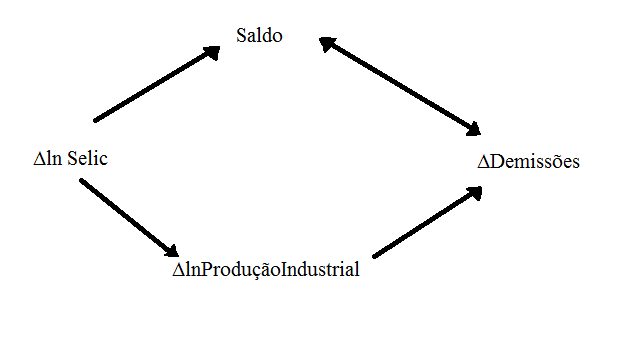
\includegraphics[width=10cm]{relacoes}}{\tiny\par}
\end{frame}
\selectlanguage{american}%


\subsection{Conditional Model for one unit}
\begin{frame}{\foreignlanguage{english}{Vale do Para�ba}}

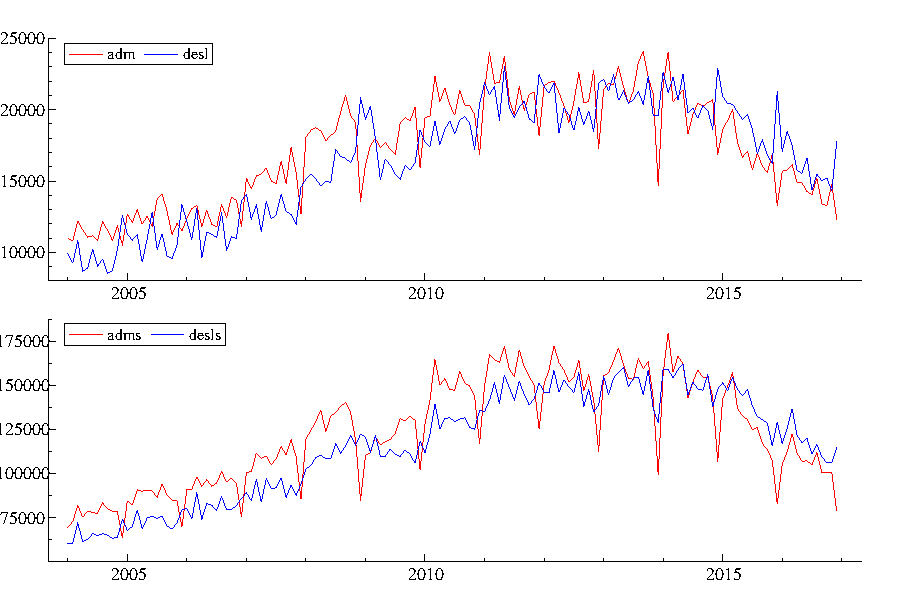
\includegraphics[width=8cm]{vale-paraiba}
\begin{itemize}
\item Admissions and dismissal cointegrate.
\end{itemize}
\end{frame}

\begin{frame}{\foreignlanguage{english}{Do they cointegrate?}}

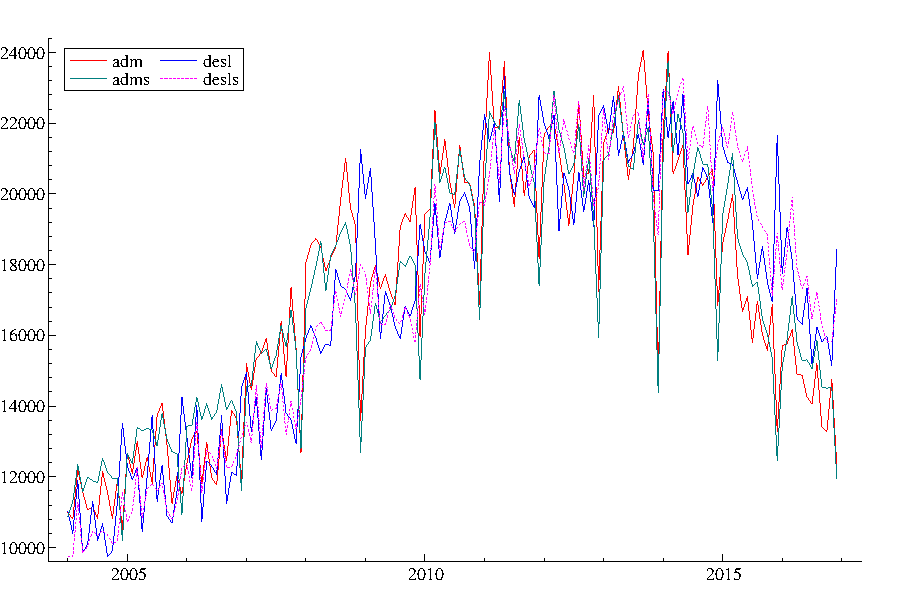
\includegraphics[width=8cm]{vale-paraiba-escala}
\begin{itemize}
\item But more than two cointegrated vectors!
\end{itemize}
\end{frame}

\begin{frame}{\foreignlanguage{english}{Conditional model for Admissons: Vale do Para�ba}}
\begin{itemize}
\item Starting Point:
\begin{itemize}
\item VARX with twelve lagas for all variables plus error correction terms;
\item Centered Seasonal Dummies;
\end{itemize}
\item Possible overfitting;
\end{itemize}
\end{frame}

\begin{frame}{\foreignlanguage{english}{Final model conditional model for Dismissals: Vale do Para�ba}}

{\scriptsize{}$\begin{array}{lcl}
\text{Dadm} & = & \ -\!\begin{array}[t]{r}
0.1615\\
^{(0.0423)}
\end{array}\text{Dadm}_{t-1}\ -\!\begin{array}[t]{r}
0.1213\\
^{(0.0369)}
\end{array}\text{Dadm}_{t-2}\ -\!\begin{array}[t]{r}
0.1228\\
^{(0.0607)}
\end{array}\text{saldo}_{t-1}\\
 &  & \ -\!\begin{array}[t]{r}
0.03239\\
^{(0.00998)}
\end{array}\text{saldo-adms}_{t-1}\ +\!\begin{array}[t]{r}
0.03253\\
^{(0.0103)}
\end{array}\text{saldo-desls}_{t-1}\ +\!\begin{array}[t]{r}
0.1146\\
^{(0.00568)}
\end{array}\text{Dadms}_{t}\\
 &  & \ +\!\begin{array}[t]{r}
0.001022\\
^{(0.00875)}
\end{array}\text{Ddesls}_{t}\ +\!\begin{array}[t]{r}
0.01186\\
^{(0.00437)}
\end{array}\text{Dadms}_{t-7}\ -\!\begin{array}[t]{r}
0.02118\\
^{(0.00811)}
\end{array}\text{Ddesls}_{t-3}\\
 &  & \ +\!\begin{array}[t]{r}
1039\\
^{(238)}
\end{array}\text{CSeasonal}_{t-10}\ +\!\begin{array}[t]{r}
2268\\
^{(550)}
\end{array}\text{DI:2012(11)}_{t}\ +\!\begin{array}[t]{r}
1710\\
^{(518)}
\end{array}\text{DI:2013(9)}_{t}\\
 &  & \ -\!\begin{array}[t]{r}
94.59\\
^{(304)}
\end{array}
\end{array}$}{\scriptsize\par}
\begin{itemize}
\item ``Global Factors'' explain part of the dynamics of admissions;
\end{itemize}
\end{frame}

\begin{frame}{\foreignlanguage{english}{Conditional model for Admissons: Vale do Para�ba}}

\selectlanguage{english}%
\textrm{\scriptsize{}
\[
\begin{array}{lcl}
\text{Ddesl} & = & \ -\!\begin{array}[t]{r}
0.2092\\
^{(0.0462)}
\end{array}\text{Dadm}_{t-1}\ -\!\begin{array}[t]{r}
0.1881\\
^{(0.0403)}
\end{array}\text{Dadm}_{t-2}\ +\!\begin{array}[t]{r}
0.4811\\
^{(0.0663)}
\end{array}\text{saldo}_{t-1}\\
 &  & \ +\!\begin{array}[t]{r}
0.06565\\
^{(0.0109)}
\end{array}\text{saldo-adms}_{t-1}\ -\!\begin{array}[t]{r}
0.06865\\
^{(0.0113)}
\end{array}\text{saldo-desls}_{t-1}\ -\!\begin{array}[t]{r}
0.03675\\
^{(0.00621)}
\end{array}\text{Dadms}_{t}\\
 &  & \ +\!\begin{array}[t]{r}
0.1568\\
^{(0.00955)}
\end{array}\text{Ddesls}_{t}\ +\!\begin{array}[t]{r}
0.01593\\
^{(0.00477)}
\end{array}\text{Dadms}_{t-7}\ -\!\begin{array}[t]{r}
0.02962\\
^{(0.00886)}
\end{array}\text{Ddesls}_{t-3}\\
 &  & \ -\!\begin{array}[t]{r}
209.2\\
^{(260)}
\end{array}\text{CSeasonal}_{t-10}\ +\!\begin{array}[t]{r}
433.5\\
^{(601)}
\end{array}\text{DI:2012(11)}_{t}\ +\!\begin{array}[t]{r}
409.8\\
^{(566)}
\end{array}\text{DI:2013(9)}_{t}\\
 &  & \ -\!\begin{array}[t]{r}
216.3\\
^{(332)}
\end{array}
\end{array}
\]
}{\scriptsize\par}
\selectlanguage{american}%
\begin{itemize}
\item ``Global Factors'' also explain part of the dynamics of dismissals;
\end{itemize}
\end{frame}

\begin{frame}{\foreignlanguage{english}{Good results on specification tests}}
\begin{itemize}
\item Vector AR 1-7 test: F(28,230) = 1.6157 {[}0.0306{]}{*} 
\item Vector Normality test: Chi\textasciicircum 2(4) = 9.7889 {[}0.0441{]}{*} 
\item Vector Hetero test: F(69,350) = 1.3114 {[}0.0619{]} 
\item Vector Hetero-X test: F(204,216)= 1.2511 {[}0.0524{]} 
\item Vector RESET23 test: F(8,250) = 1.0066 {[}0.4315{]} 
\end{itemize}
\end{frame}

\begin{frame}{\foreignlanguage{english}{Putting all the pieces together}}
\begin{itemize}
\item Solving the model using GVAR under this approach;
\item We can simulate how changes on variables such interest rate will affect
employment at regional level;
\item And forecast them as well;
\end{itemize}
\end{frame}


\section{Conclusions}
\begin{frame}{Some tentative conclusions}
\begin{itemize}
\item South, Southeast and Northeast have shown a stronger response to shocks
in Brazilian aggregate industrial production;
\item Macro factor does not play strong influence on North and Central meso
regions;
\item Formal employment will tend to recover slowly in Brazil in near future
unless high growth rates start to be observed;
\end{itemize}
\end{frame}


\appendix

\section*{}
\end{document}
